\documentclass[]{article}

\usepackage{tikz}
\usepackage{amsmath}
\usepackage{upgreek}
\usetikzlibrary{shapes,arrows,positioning,calc}
\usepackage{float}
%opening
\title{Cnstraint belief dynamics and heterogeneous mean field model}
\author{Atiyab}

\begin{document}

\maketitle

\begin{abstract}

\end{abstract}

These notes are meant to be an attempt to model the constraint belief dynamics that we encounter in the problem solving Agent Based Model (ABM). The theory is inspired by the block based epidemiological models. 

\section{The Model and prerequisites}

Before we start doing analytical modeling of the agent based model, we should start with some notations and prerequisites. We will not be discussing the ABM in detail here, but we will be discussing some terminologies and some required notations moving forward.

So, in the ABM, each agent has two attributes. An agent $(i)$ has a belief store vector with their beliefs $(\vec{B}_i)$, the opinion vector $(\vec{x}_i)$. There are total $N$ agents or people in the model. That is, $i=\left(1,2,\cdots,N-1,N\right)$. The agents are solving at any moment of time, problems involving $K$ binary variables. i.e. They can have an opinion on $k$ binary `problems'. That is, $\vec{x}_i \in \left\{0,1\right\}^K$. The information required to make decisions is in the form of boolean constraints. The constraint can be of two types, AND and XOR. So, for $k$ random variables, there can be $K(K-1)/2$ types of constraints of each type (AND or XOR). Or, there can be $K(K-1)$ total possible constraints. Together they create the set of all possible constraints that define the `Universe' ($\mathcal{U}$). 

The whole universe of constraint are not active at the same time. A subset of the universe of constraint creates the ``active" environment ($C$), $C \subset \mathcal{U}$.

This set of constraints defines the problems the agents are trying to solve at any time. The size of the environment is $|C|=M=\alpha K$ where $\alpha$ is a parameter of the model.

Agent Belief store is also a subset of the universe of constraints, $B_i \subseteq \mathcal{U}$, but note that it can include beliefs that are not active, that is, $$B_i = \{ C_1^{(i)},C_2^{(i)} , \cdots C_{2M}^i\}, \ |B_i| \le 2M.$$ 

For each constraint $C_j$ in $\vec{B}_i$, we have $\sigma_i(C_j) = {+1,-1}$. $\sigma_i(C_j)=1$ implies that the agent $i$ believes $C_j \in C$, whereas if $\sigma_i(C_j)=-1$, then the agent believes that the constraint $C_j$ is not in the environment.

\section{Creating the model}

\subsection{The blocks}

\begin{figure}[H]
	\centering
	\tikzset{
		block/.style={draw, fill=white, rectangle, minimum height=3em, minimum width=3em},
		input/.style = {coordinate},
	}
	\begin{tikzpicture}[auto, node distance=3cm, >=latex']
	\node[input, name=input] (input) {};
	\node [block, right of=input,node distance=1.5cm] (T) {$T_k(t)$};
	\node [block, right of=T] (S) {$S_k(t)$};
	\node [block, below right of=T] (N) {$N_k(t)$};
	\draw [->] (input) --node{$D_k$} (T);
	\draw [->] (T) --node{$R_k$} (S);
	\draw [->] (S) --node{$\phi_k$} (N);
	\end{tikzpicture}
\end{figure}

We start with defining the blocks for the constraints and their beliefs. We will be working with $k$-degree classes which was what we did for the mean field model. 

We define $T_k(t)$ as the fraction of live positive beliefs held by an agent of degree class $k$. i.e. an agent believes a clause $c$ exists and $c \in C(t)$. $S_k(t)$ is the fraction of stale positive beliefs held by a degree-$k$ agent and $N_k(t)$ is the fraction of live clauses that agent believe not to be true i.e. agent believes $c \notin C(t)$. 

\begin{eqnarray*}
	T_k(t)&=& \frac{\mathrm{number \ of \ live \ clauses \ believed \ to \ be \ +ve \ by\  degree \ k-agents}}{M}\\
	S_k(t)&=& \frac{\mathrm{number \ of \ retired \ clauses \ still \ believed \ to \ be \ +ve \ by\  degree \ k-agents}}{M}\\
	N_k(t)&=& \frac{\mathrm{number \ of \ clauses \ believed \ not\ to \ exist \ by\  degree \ k-agents}}{M}	
\end{eqnarray*}

The last block $N_k(t)$ does not particilate in the greedy optimisation algorithm.

The total beliefs held by an agent of degree $k$ is thus, 
$$
B_k(t)=T_k(t)+S_k(t)+N_k(t)
$$

$B_{max}=2$, since $B_i(t)$ has max capacity $2M$, this matters because once an agent is full, new beliefs must replace the older ones. 

\subsection{The flows}

Now that we have defined the blocks, in this section we define the flows between the blocks. 

\subsubsection{Private learning}

With probability $1/2$, a new clause is added to the belief set. A new clause $c$ is sampled from the universe ($\mathcal{U}$) uniformly.


Therefore the probability of sampling from $\mathcal{U} = \frac{1}{|\mathcal{U}|}=\frac{1}{K(K-1)}$.

If $T$ is the fraction of live beliefs that are known to be true, then $1-T$ is the fraction of beliefs which we know still ``exists" but has not been discovered yet. Thus, for degree $k$ class,

\begin{equation}
	D_k=\frac{1-T_k}{2|\mathcal{U}|}=\frac{1-T_k}{2K(K-1)}
	\label{eq:D_k}
\end{equation}

\subsubsection{Retiring rate}

Every $\tau$ steps, one of the $M$ clauses gets replaced by a new one. 

The risk of each clause getting replaced $= \frac{p_\tau}{M}=\frac{1}{M\tau}$, where $p_\tau$ is the time rate of clause update. Therefore, the flow ot $T_k$ retiring is:

\begin{equation}
	R_k=\frac{T_k}{M\tau}
\end{equation}
Since, removal of clause from $C(t)$, it implies that the change from $T_k\rightarrow S_k$ is $+R_k$ and the change in $S_k$ is $-R_k$.

\subsubsection{Checking rate}

Lastly, an agent with probability 1/2, an agent checks its own beliefs with the live clauses. 
Fraction of belief set which is stale is $\frac{S_k}{B_k}$. Therefore, the probability of selecting a stale belief is $\frac{1}{2}\frac{S_k}{B_k}$ and thus the flow from stale to negative is defined as:

\begin{equation}
	{\phi_k}=\frac{S_k}{2MB_k}
\end{equation}

\subsubsection{Communication}

Communication is a little more involved, the private information flows were comparably easier. To take care of communication, we have to define degree weighted compartment fractions:

\begin{equation}
	\gamma_{\!_T}=\sum_l \frac{ l P(l) T_l}{\langle k \rangle};\quad \gamma_{\!_S}=\sum_l \frac{ l P(l) S_l}{\langle k \rangle};\quad\gamma_{\!_N}=\sum_l \frac{ l P(l) N_l}{\langle k \rangle},
\end{equation}
where, $P(l)$ is the degree distribution function and $\langle k \rangle$ is average degree of the graph.

We need this as the communication is degree dependent, as the agents interact with their neighbours the nodes with higher in-degree will receive more information compared to nodes with no in degree. Infact, the nodes with zero degree in the graphs will have no source of social information and will only rely on personal exploration or what we called private learning.

The ratio $\frac{\gamma_{\!_T}}{\gamma_{\!_B}}$ is the expected share of transmissable sender beliefs that are positives, i.e. the expected share of beliefs that the agents believe to be in the environment. Here, $\gamma_{\!_B}$ is the sum of all three degree weighted fractions, $\gamma_{\!_B}=\gamma_{\!_T}+\gamma_{\!_S}+\gamma_{\!_N}$.


Similarly, $\frac{\gamma_{\!_S}}{\gamma_{\!_B}}$ and $\frac{\gamma_{\!_N}}{\gamma_{\!_B}}$ are ratio of stale and negatively held beliefs that can be transmitted along the network links. These ratios are important, as the communication step is not just sharing of clauses, what is being shared becomes very important. And thus, the communication will change each of the three blocks.


Let $C_{T,k}$ be the inflow of true positive clauses from the neighborhood for agents with degree $k$.

\begin{equation}
	C_{T,k} = \beta_k \left(\frac{\gamma_{\!_T}}{\gamma_{\!_B}}\right) 
\end{equation}

Each of the blocks will have its respective inflow defined analogously.

%
%Let $C_{T,k}$ be the inflow of true positive clauses from the neighborhood for agents with degree $k$. It is defined as:
%
%\begin{equation}
%	C_{T,k} = \beta_k \left(\frac{\gamma_{\!_T}}{\gamma_{\!_B}}\right)
%\end{equation}
%Each of the blocks will have its respective inflow defined analogously.

Here, $\beta_k$ represents the available communication bandwidth, defined as:
\begin{equation}
	\beta_k = \frac{k}{M \langle k \rangle} \max\left(0, 1 - \frac{B_k}{2}\right)
\end{equation}

The first fractional term represents the structural limit of the network. The second term, included in a maximum function, enforces the strict physical memory constraint of the agent. Remember each agent can only have $B_{max}=2$, so we enforce this as a carrying capacity of the dynamics.

Since, $\dot(B_k)=\dot{T_k}+\dot{S_k}+\dot{N_k}$, the $\dot{B_k}$ needs a product term having $(1-B_k/2)$. This ensures $B_k$ has an attractor at $B_k=2$ and provides a containing effect to the total clauses. Without this term, the total beliefs can explode as our mean field has a positive inflow. 

\subsection{Final Blocks and model}

\begin{figure}[H]
	\centering
	\tikzset{
		block/.style={draw, fill=white, rectangle, minimum height=3em, minimum width=3em},
		input/.style = {coordinate},
	}
	\begin{tikzpicture}[auto, node distance=3cm, >=latex']
		\node[input, name=input] (input) {};
		
		% Reduced node distance to 1.5cm to shorten the left inflow arrow
		\node [block, right of=input, node distance=1.5cm] (T) {$T_k(t)$};
		\node [block, right of=T] (S) {$S_k(t)$};
		\node [block, below right of=T] (N) {$N_k(t)$};
		
		% Define starting coordinates for the new dashed arrows
		\node [input, above of=T, node distance=1.5cm] (topT) {};
		\node [input, above of=S, node distance=1.5cm] (topS) {};
		\node [input, left of=N, node distance=1.5cm] (leftN) {};
		
		% Original solid arrows
		\draw [->] (input) --node{$D_k$} (T);
		\draw [->] (T) --node{$R_k$} (S);
		\draw [->] (S) --node{$\phi_k$} (N);
		
		% New dashed arrows with labels
		\draw [->, dashed] (topT) -- node[right] {$C_{T,k}$} (T);
		\draw [->, dashed] (topS) -- node[right] {$C_{S,k}$} (S);
		\draw [->, dashed] (leftN) -- node[above] {$C_{N,k}$} (N);
	\end{tikzpicture}
	\caption{Final Block model showing all the flows and the three blocks for true positives, stale beliefs and the negatively held beliefs}
\end{figure}

Now that we have defined the blocks, we can combine all the flows to write the final differential equations
\begin{eqnarray}
	\frac{dT_k}{dt}&=& D_k + C_{T,k} - R_k \\
	\frac{dS_k}{dt}&=& R_k + C_{S,k} - \phi_k\\
	\frac{dN_k}{dt}&=& \phi_k + C_{N,k} \\
	\frac{dB_k}{dt}&=& D_k + C_{T,k} + C_{S,k} + C_{N,k}=\dot{T_k}+\dot{S_k}+\dot{N_k}\nonumber
\end{eqnarray}

\subsection{Decision making?}

What about decision making? In the heterogenous mean field model, we had derived the following differential equation to for the fraction of $1$ in agents of a degree class $k$ as $((p_k)$:

$$
\frac{dp_k}{dt}=R_k\left[(1-p_k)Pr(Z(\Theta>0)) -p_k Pr (Z(\Theta)<0)\right]
$$

Here, $R_k= 2\lambda\frac{k}{\langle k \rangle}$, $Z=Y-X_1=A_1+X_0-X_1$, $X_1$ were the number of XOR clauses  where the partner is zero. and $A_1$ was the number of AND clauses where the partner is 1. 
$\Theta$ is the degree weighted $p_k$, defined as $\Theta=\sum_l \frac{l P_l p_l}{ \langle k \rangle }$ and finally $p_k=Pr(x_i=1|k)$ is the expected voting assignment to $1$ for an agent of degree $k$. 

Now, to calculate $A_1$, $X_0$, and $X_1$, the agent evaluates potential flips using only the positively believed clauses $T_k(t) \cup S_k(t)$.

Subsequently, the static parameter $\alpha$ is no longer valid. The Poisson means for evaluating $Z(\Theta)$ must be driven by the time-dependent effective constraint density,

\begin{equation}
	\alpha_{\text{eff}, k}(t) = \alpha \left( T_k(t) + S_k(t) \right)
\end{equation}

The generic network interaction rate $R_k$ is no longer active. Because agents execute the greedy optimization strictly upon the successful acquisition of a positive belief, the voting rate must be dynamically coupled to the inflows of positive clauses:

\begin{equation}
	\frac{dp_k}{dt} = 2 c_t M \left(D_k + C_{T,k} + C_{S,k}\right) \left[ (1-p_k)\Pr(Z > 0) - p_k\Pr(Z < 0) \right]
\end{equation}

where $c_t$ handles the continuous-time calibration, and the probability distributions defining $Z$ are parameterized by $\alpha_{\text{eff}, k}(t)$ and the global consensus $\Theta$.


\subsubsection{Result}

We simulate the 4 coupled equation ($p_k$,$T_k$,$S_k$,$N_k$) for a random network, we use a random erdos renyi network of 100 nodes and solve the equations for the network, we consider $K=30,\alpha=2,\tau=10,c_t=0.01$. We fix the $c_t$ as small. Right now it is fixed as 0.1.

\begin{figure}[H]
	\centering
	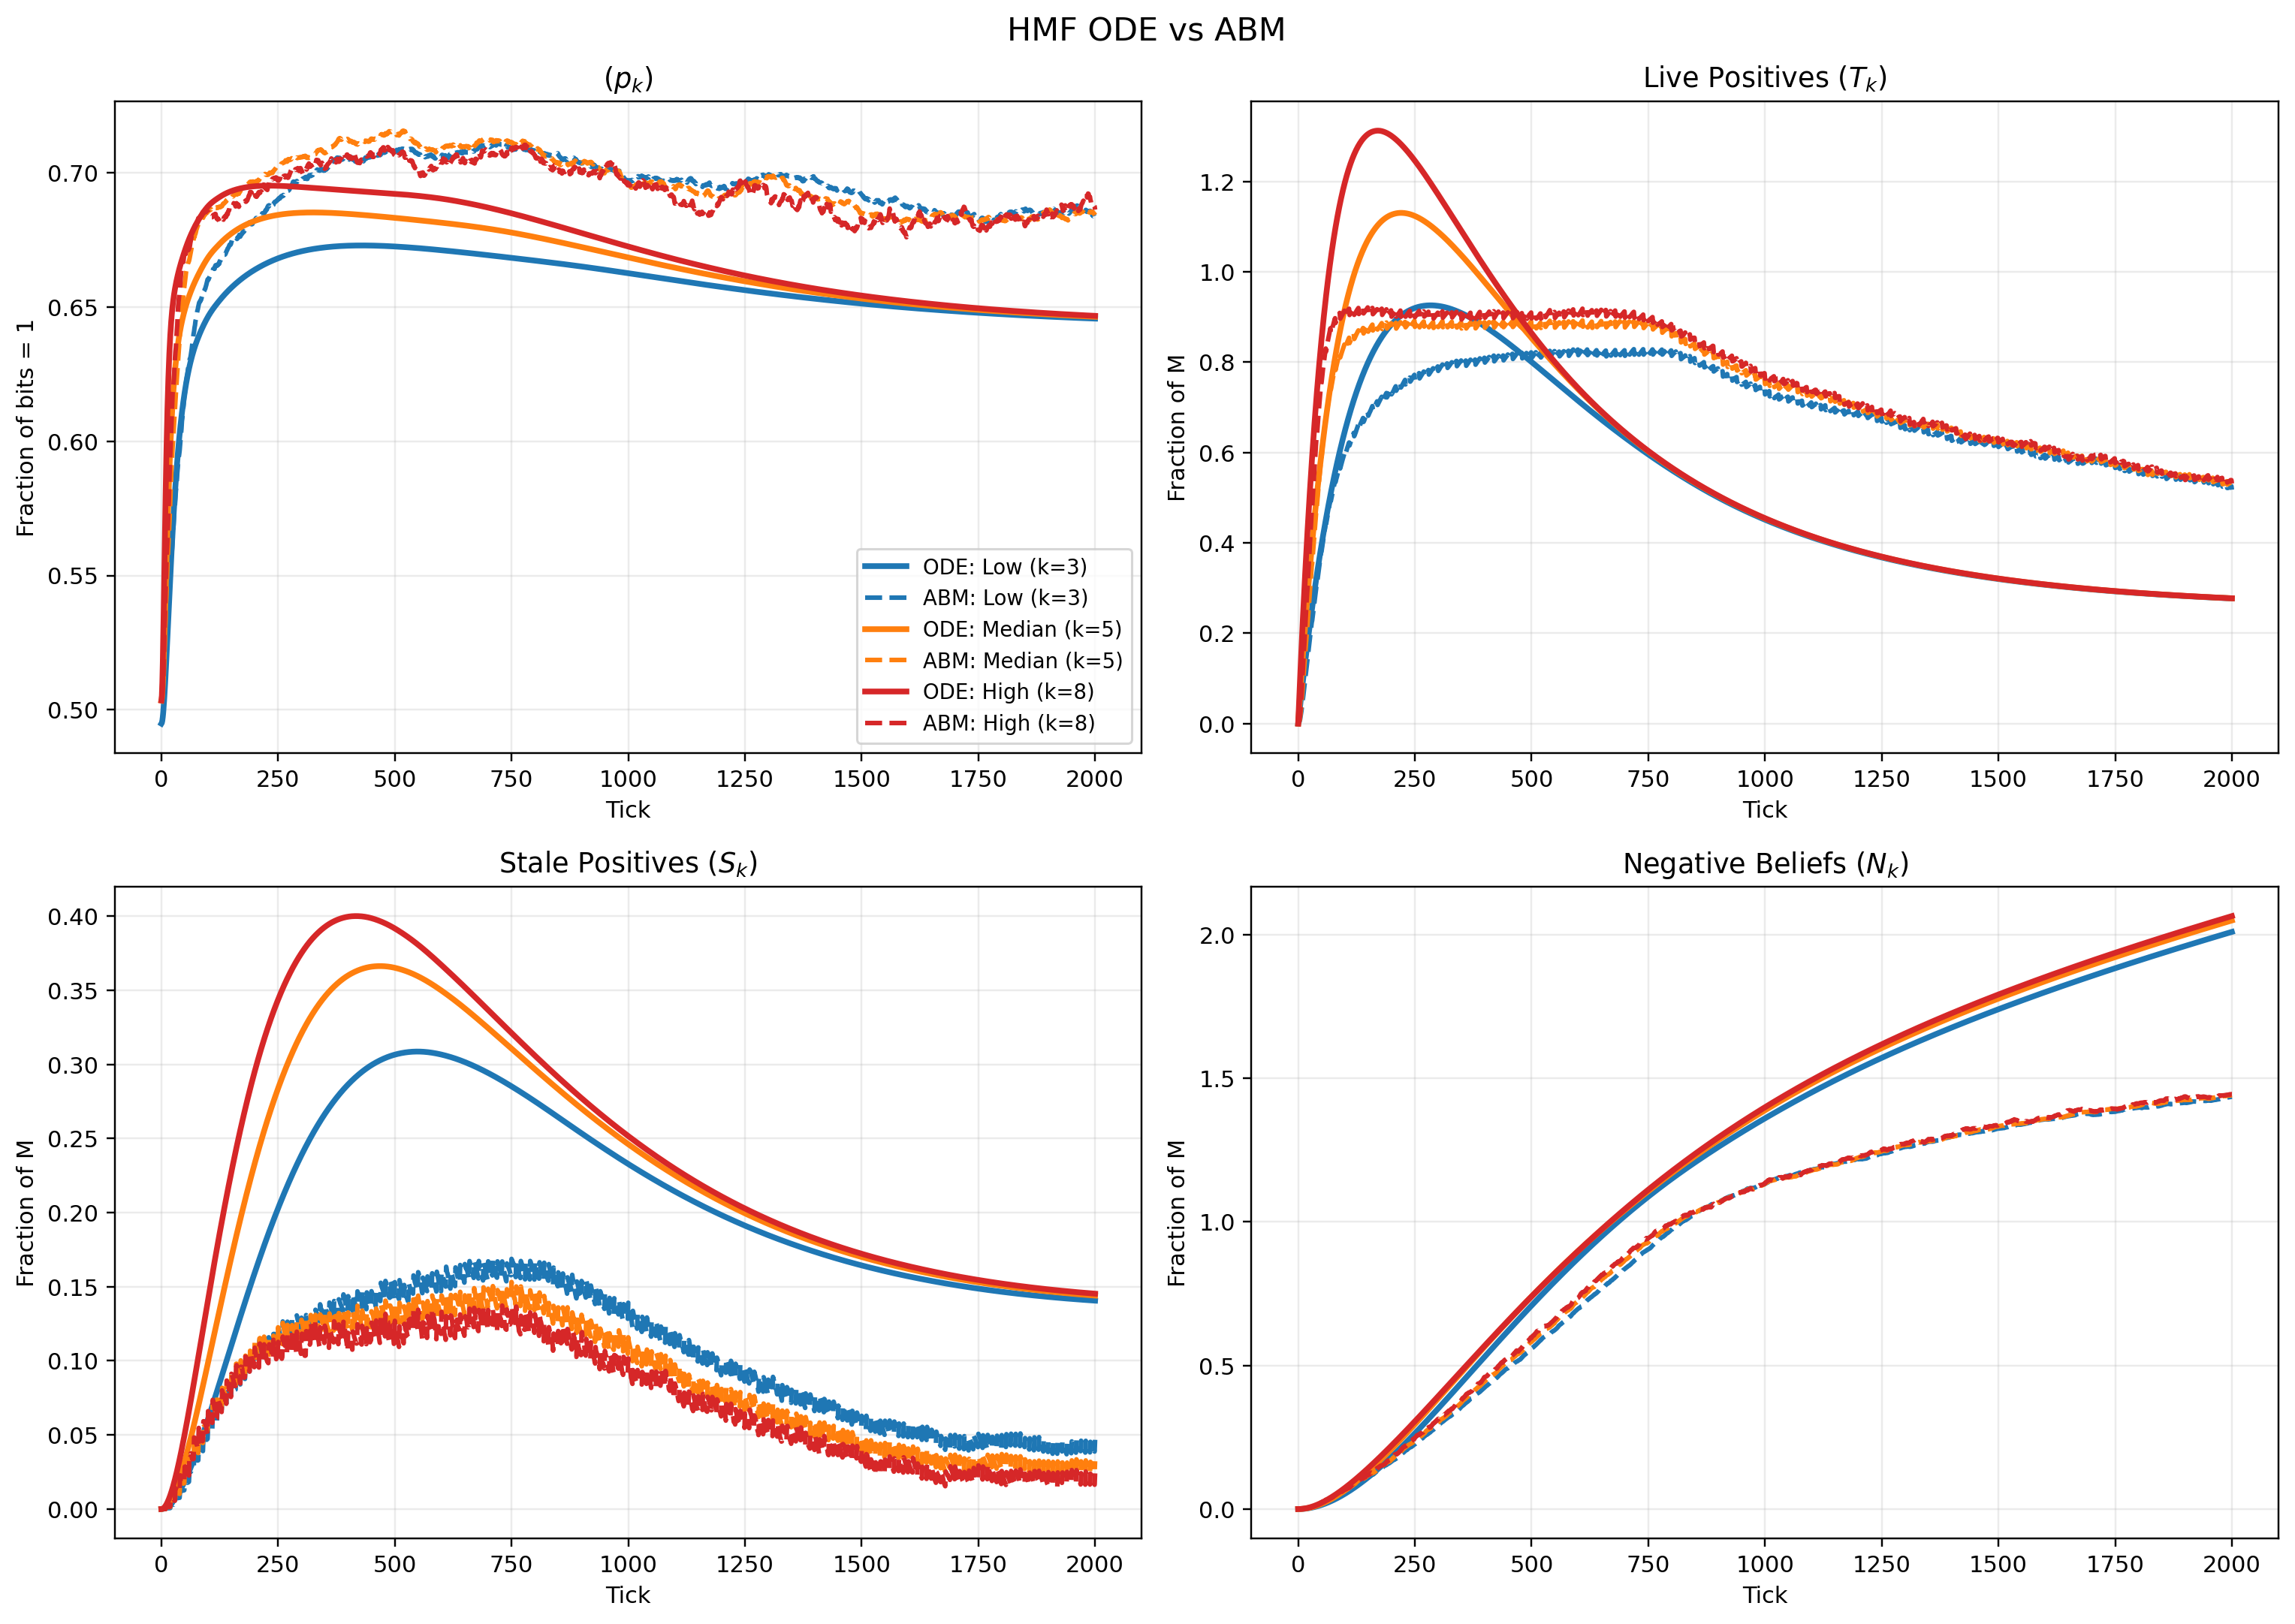
\includegraphics[width=0.75\columnwidth]{images/1_naive_model.png}
\end{figure}

Few observations, the $N_k$ fraction value goes almost to 2.0. And The number of live positives ($T_k$) goes beyond 1.0, which is impossible. We allow the maximum size of the Belief vector as $2M$, to model an agent having fake news (with $N_k$) and also old information $S_k$. But the fraction of live agents ($|C|=M$) cannot theoretically go beyond 1.

Why is this happening? Answer: lack of eviction of clauses. In the ABM, the clause that enters first, leaves first. The oldest clause in the Belief set gets removed once we reach the limit. We are missing that in the EBM.

While the $\max(0, 1 - B_k/2)$ term limits off incoming social communication as the belief store fills, it does not stop private discovery ($D_k$). 

$$
\frac{dB_k}{dt}=D_k+C_{T,k}+C{S,k}+C_{N,k}
$$
Because $D_k$ remains strictly positive, $B_k$ will artificially breach the maximum capacity of 2 unless an explicit eviction mechanism is modeled.

\subsection{Capacity and Eviction}

\begin{figure}[H]
	\centering
	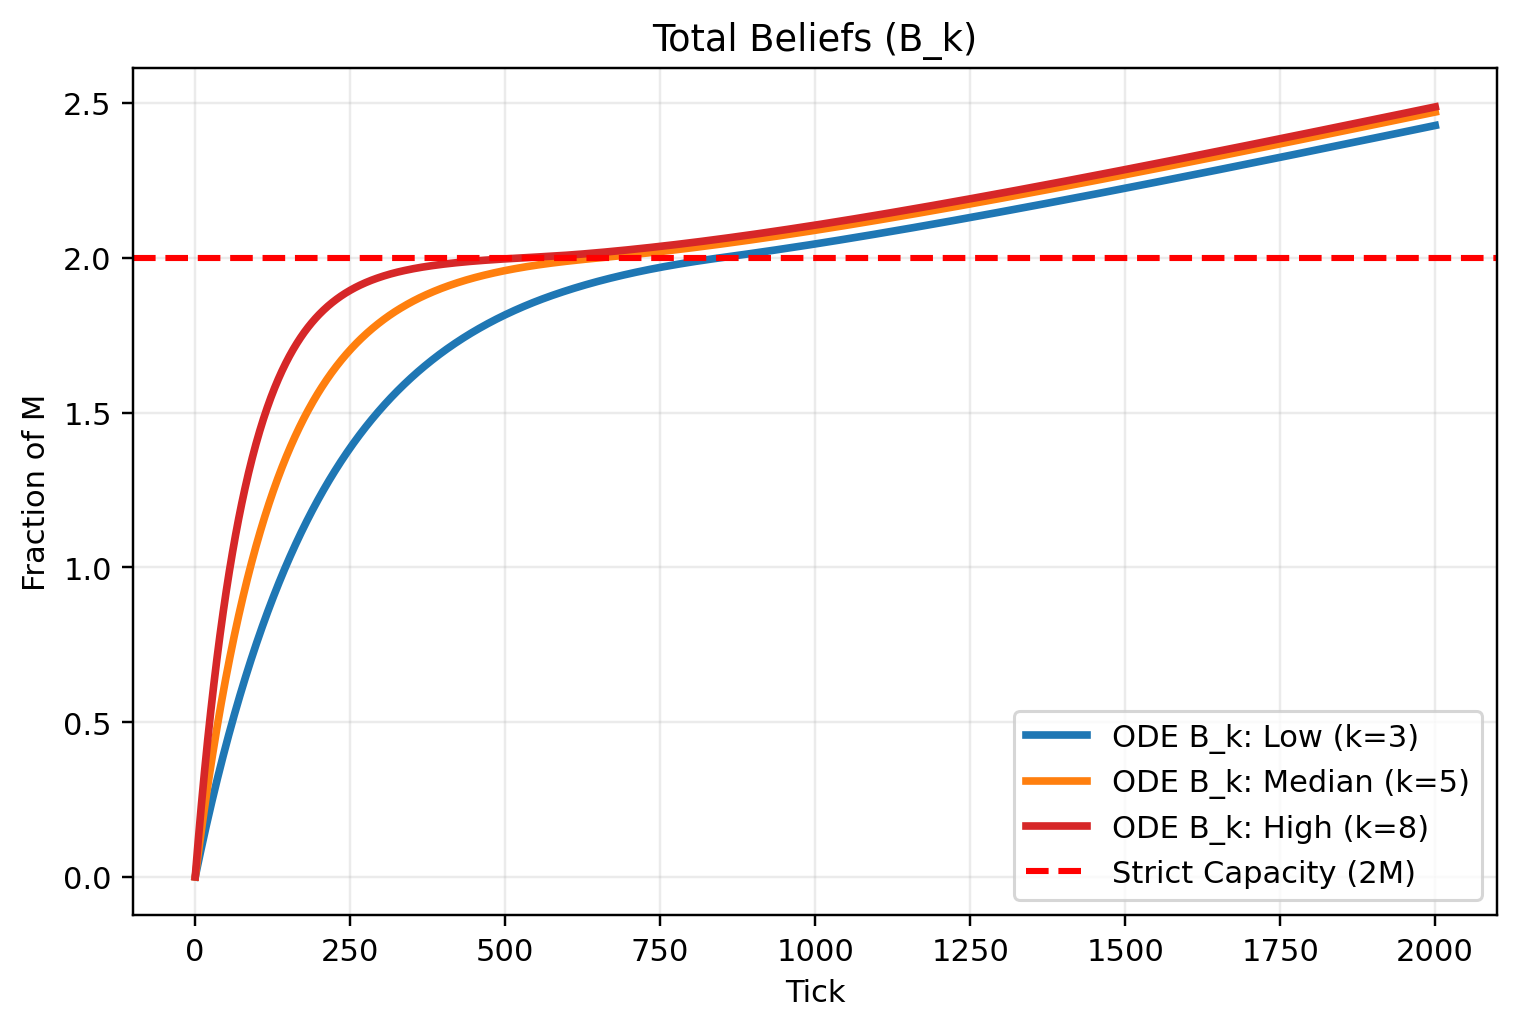
\includegraphics[width=0.75\columnwidth]{images/0_capacity_breach_proof}
\end{figure}

In the underlying ABM, overflowing memory triggers a removal of the oldest clause.To capture this continuously, we define the total information influx as $I_k = D_k + C_{T,k} + C_{S,k} + C_{N,k}$. We can introduce a smooth eviction rate $E_k$ that perfectly balances this influx as the system approaches capacity:

\begin{equation}
	E_k = \frac{I_k}{1+e^{-\kappa(\tilde{B}_k-B_0)}} 
\end{equation}

We needed a function that saturates to the input flux ($I_k$) as the physical memory approaches its limit. We use the logistic function(used in ecology), where $\tilde{B}_k = B_k / 2.0$ represents the fractional occupancy of the agent's memory. To ensure, $E_k$ reaches $I_k$ quickly, we use the slope $\kappa$ as a very high number. $B_0$ is the occupancy which it reaches at halfway point. We can use, a high $\kappa$ and use midpoint as 0.95, i.e. we say it reaches half $B$ $95\%$ of the way. This ensures that $E_k$ is low for most way and then rises steep, making sure the eviction starts happening at the end.

We allocate this eviction proportionally across the compartments,
\begin{equation}
	E_{T,k} = E_k \frac{T_k}{B_k}, \quad E_{S,k} = E_k \frac{S_k}{B_k}, \quad E_{N,k} = E_k \frac{N_k}{B_k}
\end{equation}

We also know the $T_k$ needs to be below $1$. We change the inflow rate. The probability that a broadcasted true positive is genuinely novel to the receiver is exactly $(1 - T_k)$. Thus, the effective inflow is:

\begin{equation}
	C_{T,k} = \beta_k \left(\frac{\gamma_{\!_T}}{\gamma_{\!_B}}\right) \max(0, 1 - T_k)
\end{equation}

Each of the blocks will have its respective inflow defined analogously, scaled by the probability that the incoming clause is novel. For instance, the stale inflow becomes $C_{S,k} = \beta_k (\frac{\gamma_{\!_S}}{\gamma_{\!_B}}) \max(0, 1 - \frac{S_k}{\mathcal{U}/M - 1})$.

\subsubsection{Results}

We simulate the results again now with eviction term as well. We simulate the model for the same network. The differential equations are now updated to:
\begin{eqnarray}
	\frac{dT_k}{dt}&=& D_k + C_{T,k} - R_k - E_{T,k}\\
	\frac{dS_k}{dt}&=& R_k + C_{S,k} - \phi_k- E_{S,k}\\
	\frac{dN_k}{dt}&=& \phi_k + C_{N,k} - E_{N,k}\\
	\frac{dB_k}{dt}&=& D_k + C_{T,k} + C_{S,k} + C_{N,k}- E_{T,k}- E_{S,k}- E_{N,k}=\dot{T_k}+\dot{S_k}+\dot{N_k}\nonumber
\end{eqnarray}

The results for the updated model on the same network gives us a more contained result.

\begin{figure}[H]
	\centering
	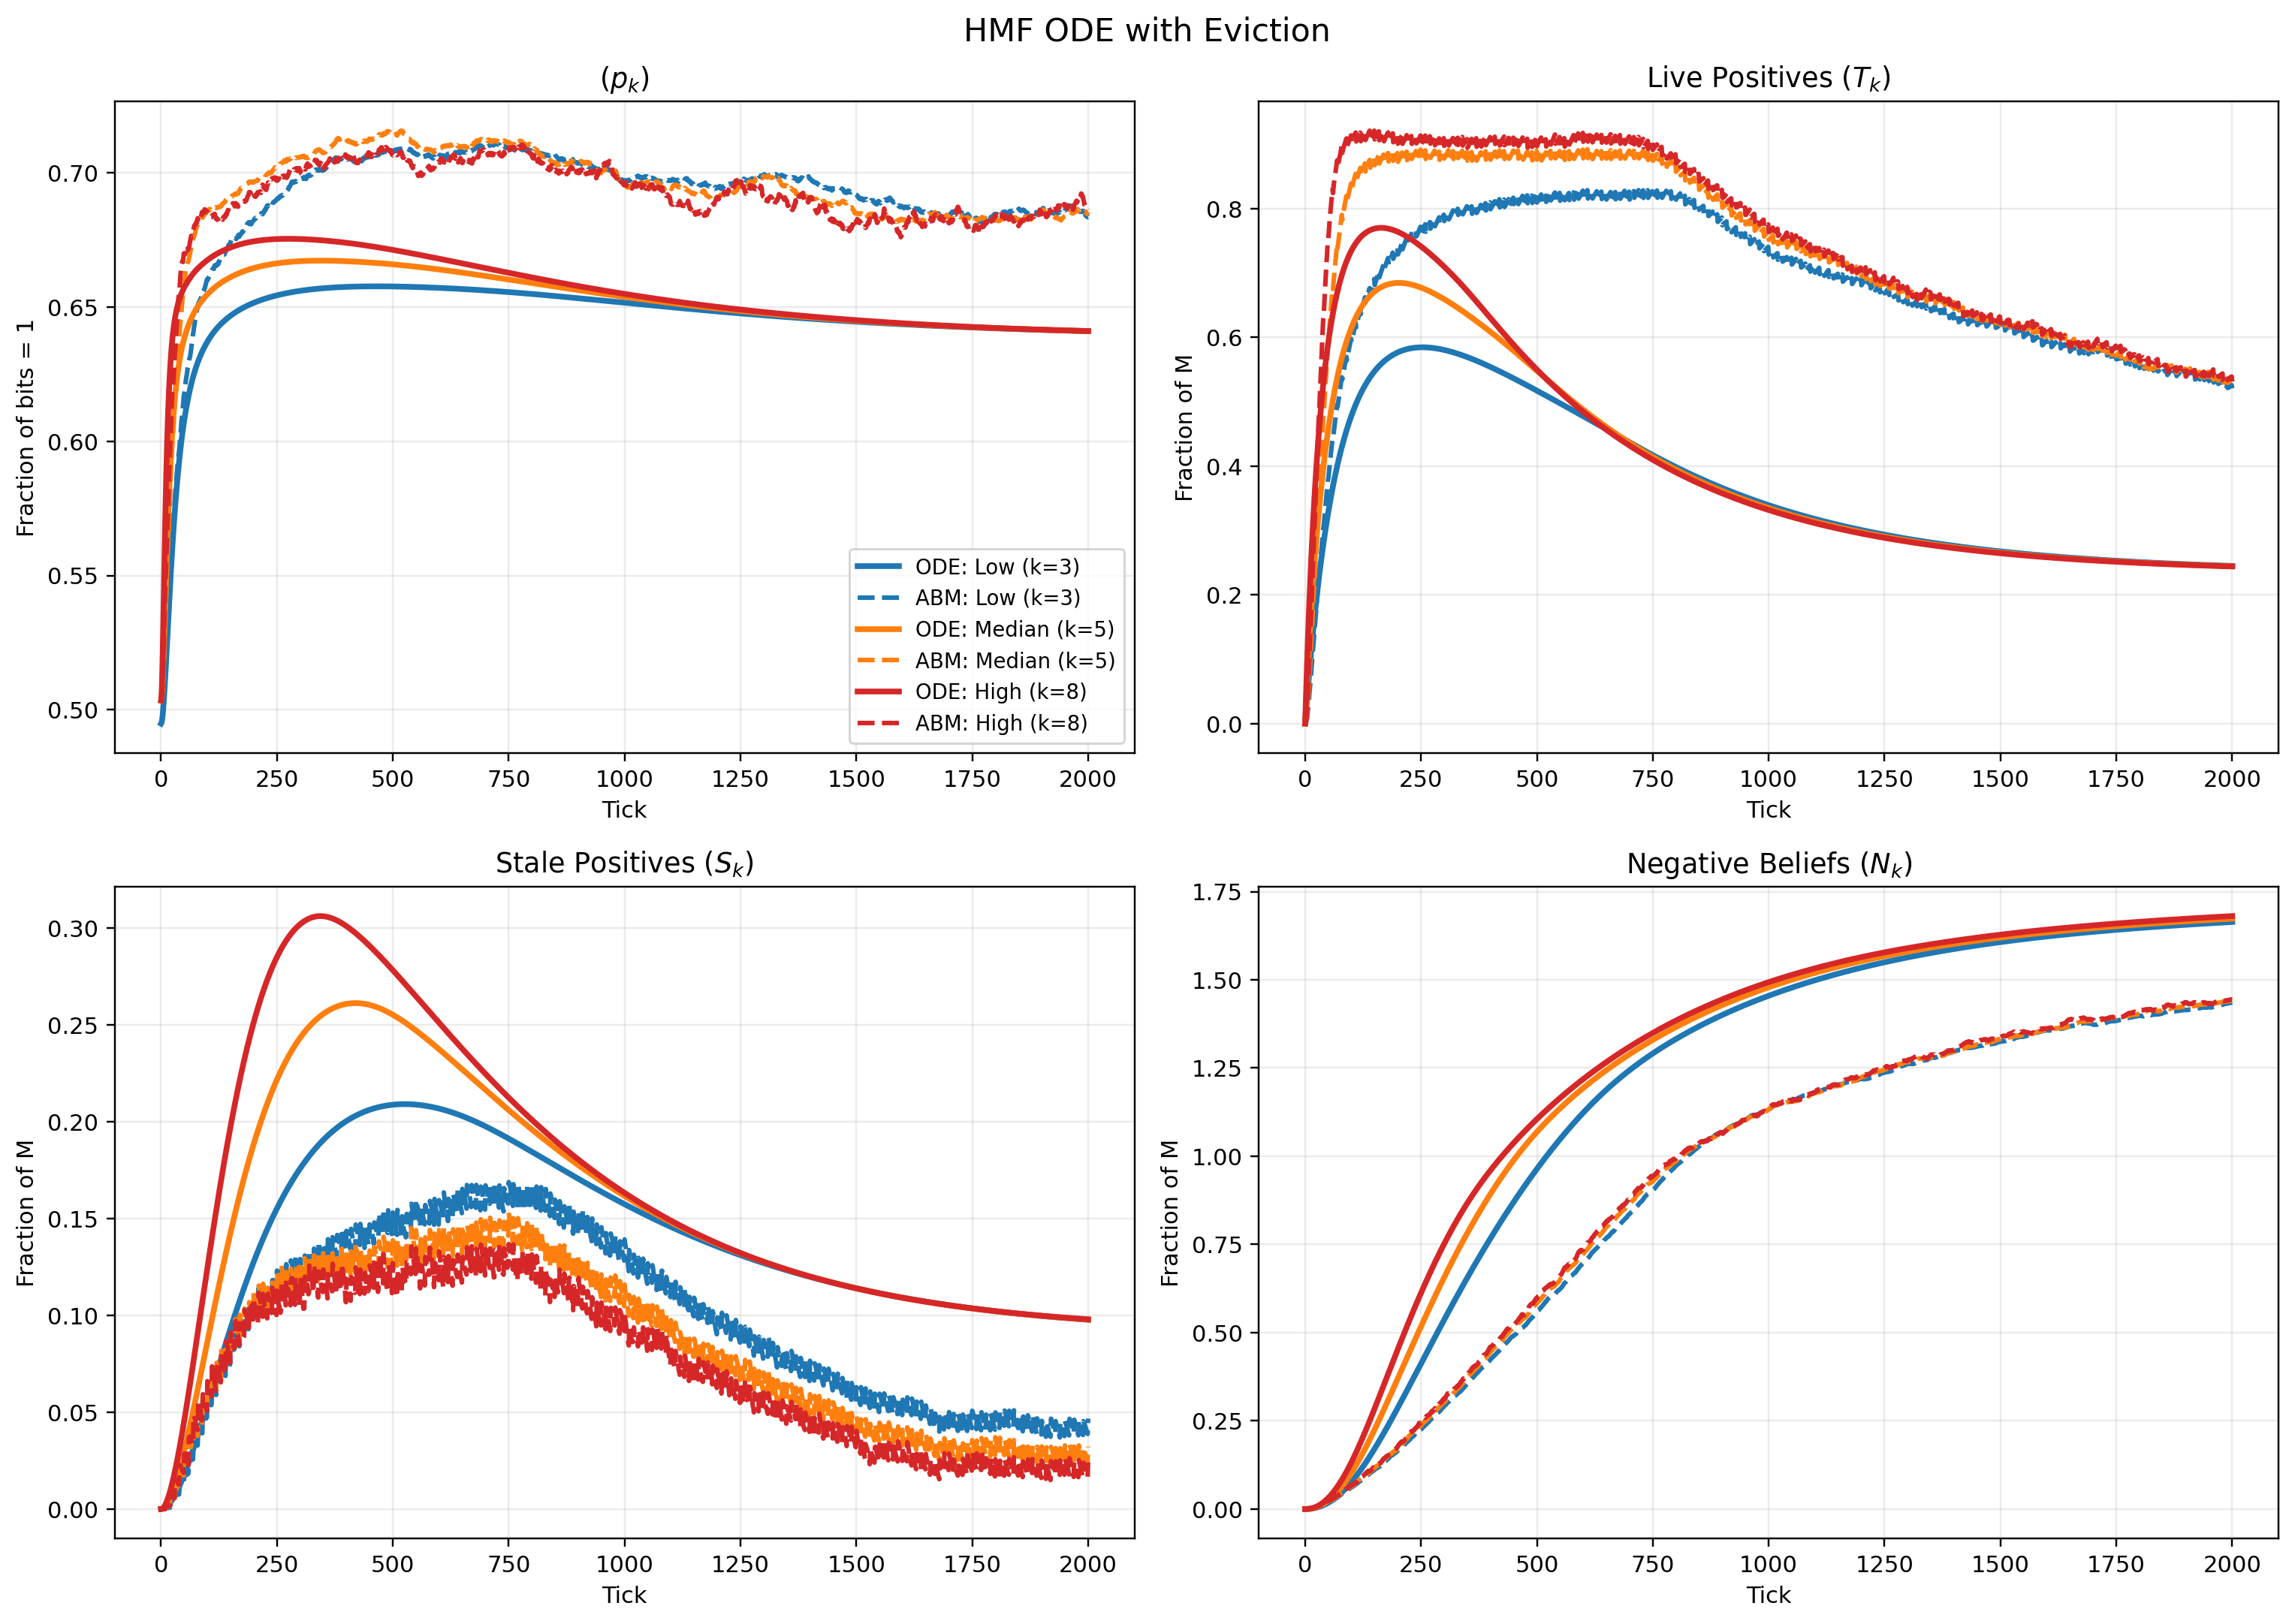
\includegraphics[width=0.75\columnwidth]{images/2_linear_limit}
\end{figure}

\subsection{Speed of constraint change}

The speed at which $T_k$ rises slower than the ABM. Something is missing?

In the agent based model, we have an additional element. If an agent receives a true positive they already hold, they simply draw again. The probability that they fail to find a novel clause is not $T_k$. It is the probability that they draw a redundant clause 10 times in a row, which is exactly $(T_k)^{10}$. Thus, the equation \ref{eq:D_k} needs to be changed with $1-T_k^{10}$.

By using $(T_k)^{10}$, the ODE will perfectly replicate the aggressive early slope of the ABM.

\subsubsection{Result}

Running the base model with eviction and the multiple draws.

\begin{figure}[H]
	\centering
	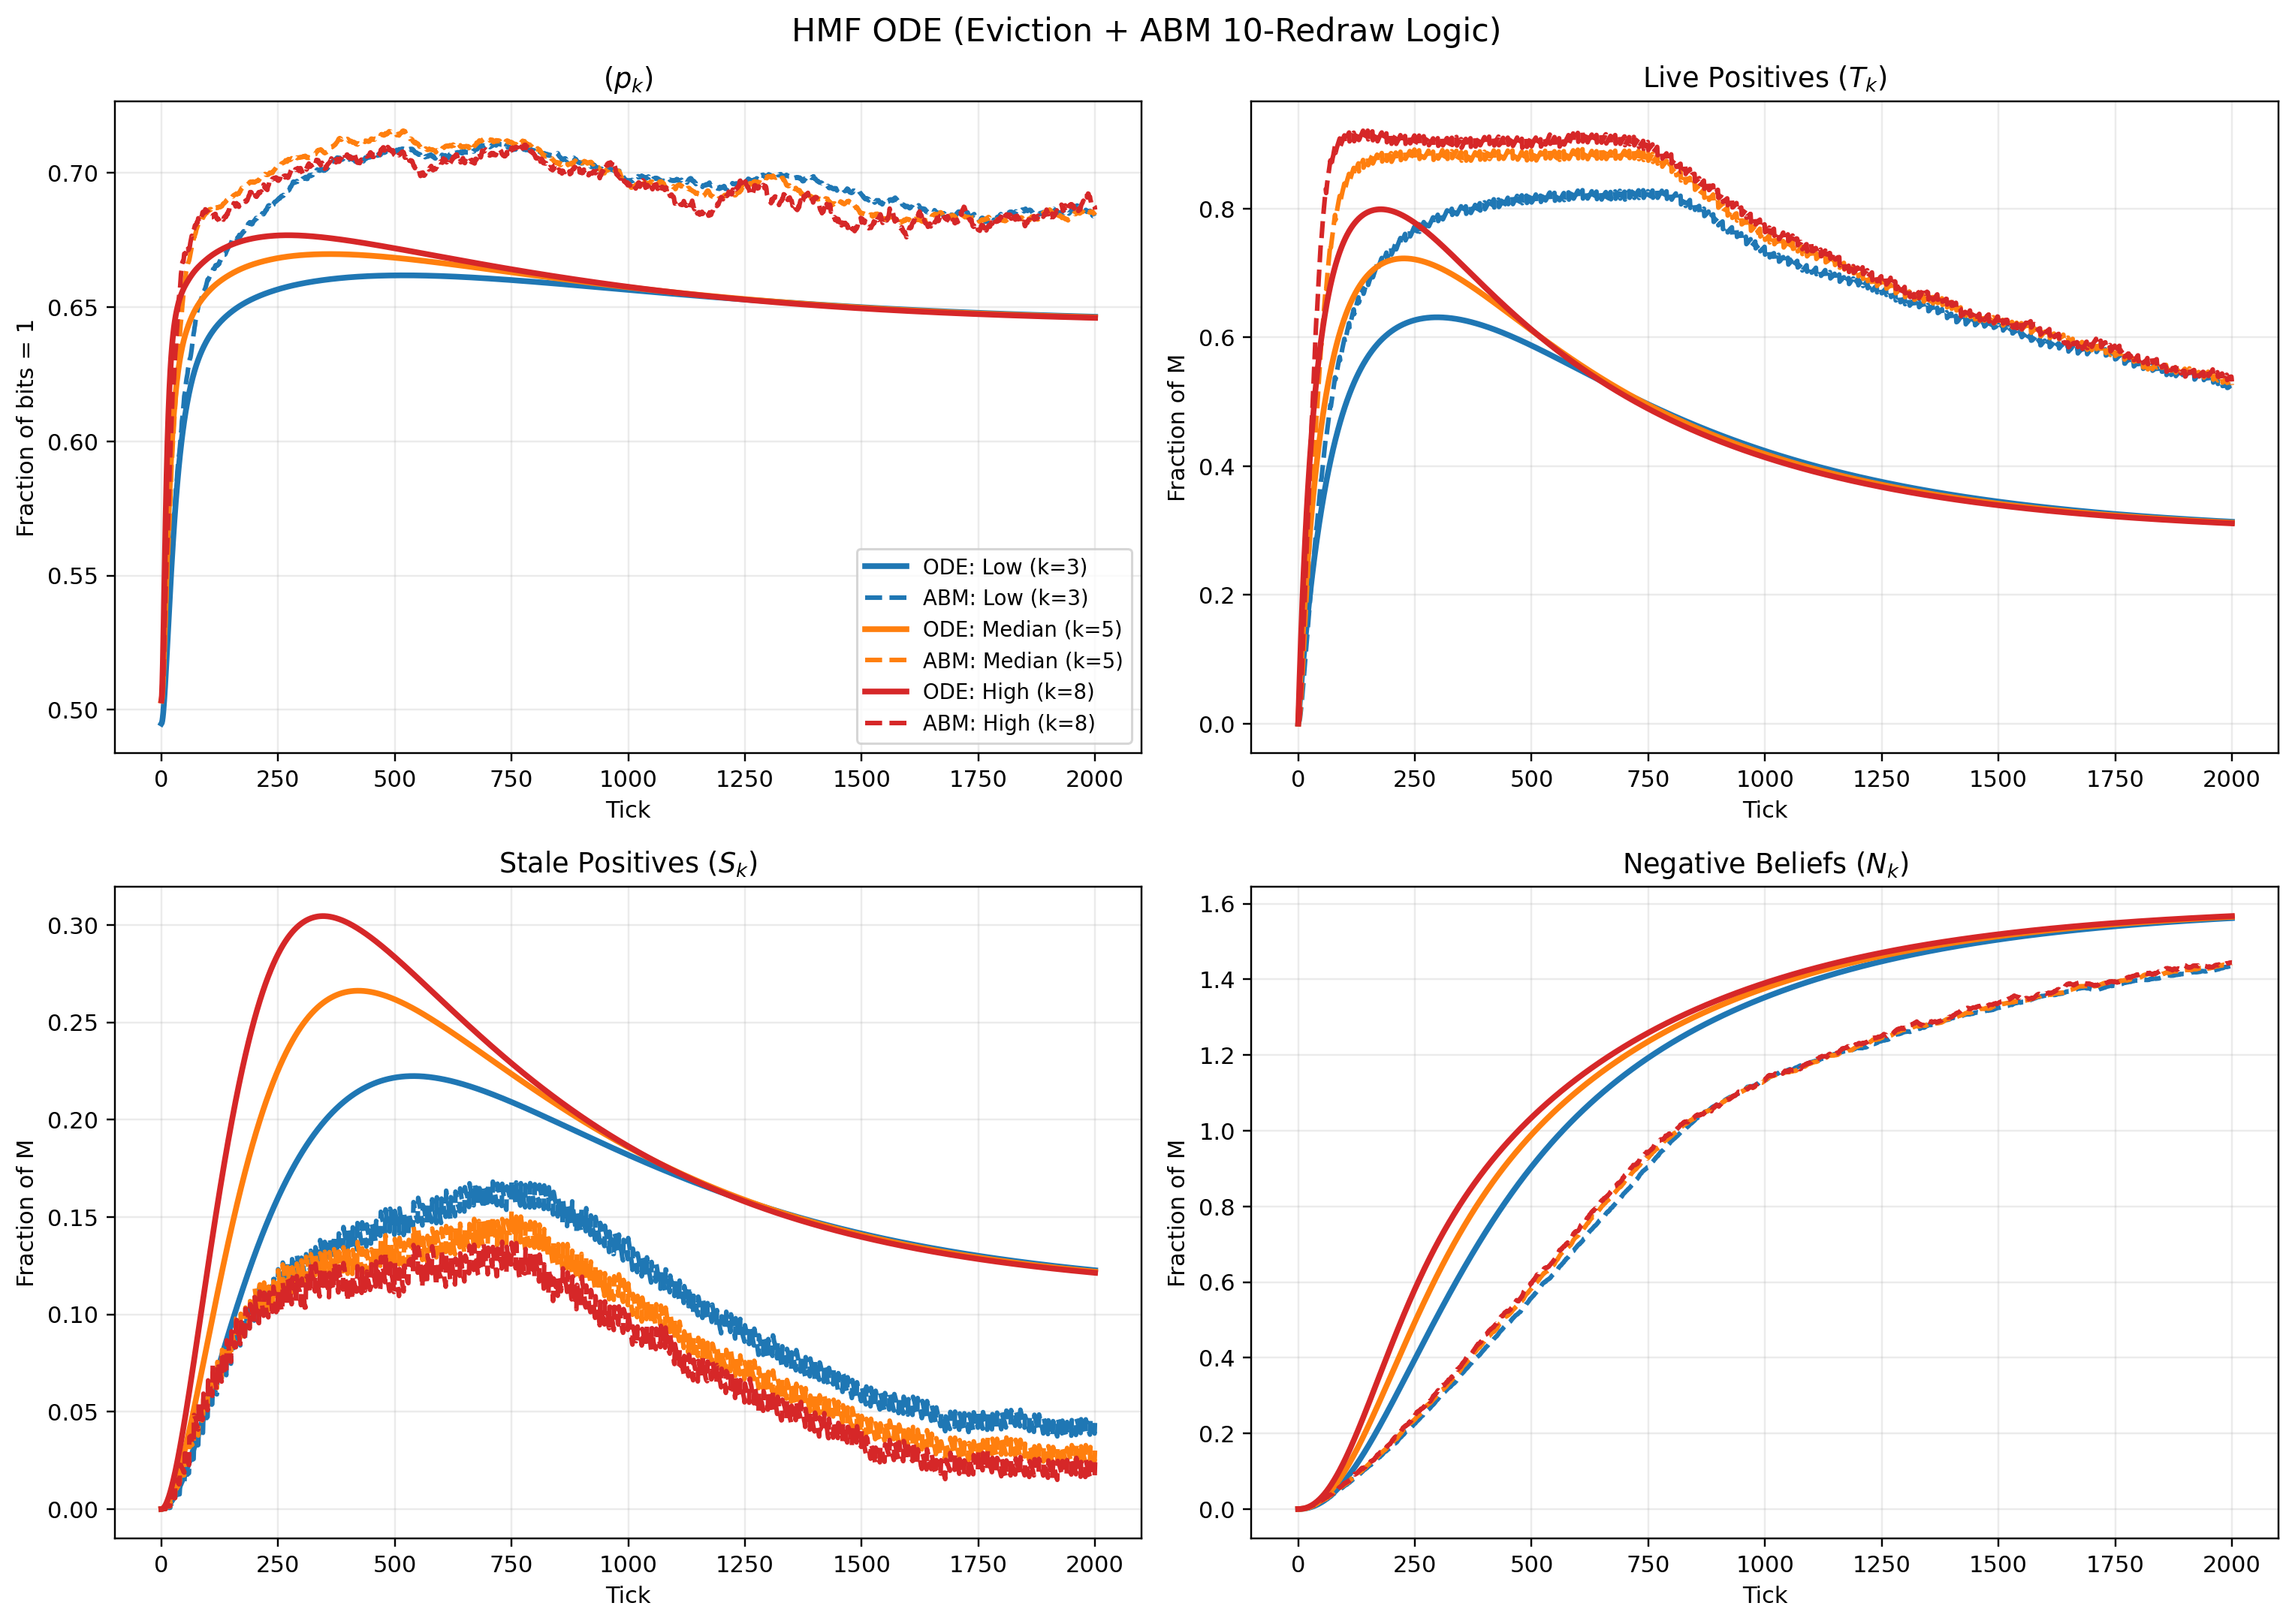
\includegraphics[width=0.75\columnwidth]{images/3_final_redraw_limit}
\end{figure}

While the equations now successfully bound the compartment capacities, a structural gap remains between the ODE and the ABM. The ODE underestimates $T_k$ and overestimates $S_k$.

Maybe, we do not need to add these more complex addition to the model. The original model already works okay and if we want to just have a theoretical model that covers most of the aspects, the first version already captures a few interesting things of the model.
\end{document}
